% Options for packages loaded elsewhere
% Options for packages loaded elsewhere
\PassOptionsToPackage{unicode}{hyperref}
\PassOptionsToPackage{hyphens}{url}
\PassOptionsToPackage{dvipsnames,svgnames,x11names}{xcolor}
%
\documentclass[
  english,
  russian,
  12pt,
  a4paper,
  DIV=11,
  numbers=noendperiod]{scrreprt}
\usepackage{xcolor}
\usepackage{amsmath,amssymb}
\setcounter{secnumdepth}{-\maxdimen} % remove section numbering
\usepackage{iftex}
\ifPDFTeX
  \usepackage[T1]{fontenc}
  \usepackage[utf8]{inputenc}
  \usepackage{textcomp} % provide euro and other symbols
\else % if luatex or xetex
  \usepackage{unicode-math} % this also loads fontspec
  \defaultfontfeatures{Scale=MatchLowercase}
  \defaultfontfeatures[\rmfamily]{Ligatures=TeX,Scale=1}
\fi
\usepackage{lmodern}
\ifPDFTeX\else
  % xetex/luatex font selection
  \setmainfont[Ligatures=Common,Ligatures=TeX,Scale=0.94]{IBM Plex
Serif}
  \setsansfont[Ligatures=Common,Ligatures=TeX,Scale=MatchLowercase,Scale=0.94]{IBM
Plex Sans}
  \setmonofont[Scale=MatchLowercase,Scale=0.94,FakeStretch=0.9]{IBM Plex
Mono}
  \setmathfont[]{STIX Two Math}
\fi
% Use upquote if available, for straight quotes in verbatim environments
\IfFileExists{upquote.sty}{\usepackage{upquote}}{}
\IfFileExists{microtype.sty}{% use microtype if available
  \usepackage[]{microtype}
  \UseMicrotypeSet[protrusion]{basicmath} % disable protrusion for tt fonts
}{}
\usepackage{setspace}
% Make \paragraph and \subparagraph free-standing
\makeatletter
\ifx\paragraph\undefined\else
  \let\oldparagraph\paragraph
  \renewcommand{\paragraph}{
    \@ifstar
      \xxxParagraphStar
      \xxxParagraphNoStar
  }
  \newcommand{\xxxParagraphStar}[1]{\oldparagraph*{#1}\mbox{}}
  \newcommand{\xxxParagraphNoStar}[1]{\oldparagraph{#1}\mbox{}}
\fi
\ifx\subparagraph\undefined\else
  \let\oldsubparagraph\subparagraph
  \renewcommand{\subparagraph}{
    \@ifstar
      \xxxSubParagraphStar
      \xxxSubParagraphNoStar
  }
  \newcommand{\xxxSubParagraphStar}[1]{\oldsubparagraph*{#1}\mbox{}}
  \newcommand{\xxxSubParagraphNoStar}[1]{\oldsubparagraph{#1}\mbox{}}
\fi
\makeatother


\usepackage{longtable,booktabs,array}
\usepackage{calc} % for calculating minipage widths
% Correct order of tables after \paragraph or \subparagraph
\usepackage{etoolbox}
\makeatletter
\patchcmd\longtable{\par}{\if@noskipsec\mbox{}\fi\par}{}{}
\makeatother
% Allow footnotes in longtable head/foot
\IfFileExists{footnotehyper.sty}{\usepackage{footnotehyper}}{\usepackage{footnote}}
\makesavenoteenv{longtable}
\usepackage{graphicx}
\makeatletter
\newsavebox\pandoc@box
\newcommand*\pandocbounded[1]{% scales image to fit in text height/width
  \sbox\pandoc@box{#1}%
  \Gscale@div\@tempa{\textheight}{\dimexpr\ht\pandoc@box+\dp\pandoc@box\relax}%
  \Gscale@div\@tempb{\linewidth}{\wd\pandoc@box}%
  \ifdim\@tempb\p@<\@tempa\p@\let\@tempa\@tempb\fi% select the smaller of both
  \ifdim\@tempa\p@<\p@\scalebox{\@tempa}{\usebox\pandoc@box}%
  \else\usebox{\pandoc@box}%
  \fi%
}
% Set default figure placement to htbp
\def\fps@figure{htbp}
\makeatother



\ifLuaTeX
\usepackage[bidi=basic,provide=*]{babel}
\else
\usepackage[bidi=default,provide=*]{babel}
\fi
\ifPDFTeX
\else
\babelfont{rm}[Ligatures=Common,Ligatures=TeX,Scale=0.94]{IBM Plex
Serif}
\fi
% get rid of language-specific shorthands (see #6817):
\let\LanguageShortHands\languageshorthands
\def\languageshorthands#1{}


\setlength{\emergencystretch}{3em} % prevent overfull lines

\providecommand{\tightlist}{%
  \setlength{\itemsep}{0pt}\setlength{\parskip}{0pt}}



 
\usepackage[style=gost-numeric,parentracker=true,backend=biber,hyperref=auto,language=auto,autolang=other*,citestyle=gost-numeric]{biblatex}
\addbibresource{bib/cite.bib}


\KOMAoption{captions}{tableheading}
\usepackage{indentfirst}
\usepackage{float}
\floatplacement{figure}{H}
\makeatletter
\@ifpackageloaded{caption}{}{\usepackage{caption}}
\AtBeginDocument{%
\ifdefined\contentsname
  \renewcommand*\contentsname{Содержание}
\else
  \newcommand\contentsname{Содержание}
\fi
\ifdefined\listfigurename
  \renewcommand*\listfigurename{Список Иллюстраций}
\else
  \newcommand\listfigurename{Список Иллюстраций}
\fi
\ifdefined\listtablename
  \renewcommand*\listtablename{Список Таблиц}
\else
  \newcommand\listtablename{Список Таблиц}
\fi
\ifdefined\figurename
  \renewcommand*\figurename{Рисунок}
\else
  \newcommand\figurename{Рисунок}
\fi
\ifdefined\tablename
  \renewcommand*\tablename{Таблица}
\else
  \newcommand\tablename{Таблица}
\fi
}
\@ifpackageloaded{float}{}{\usepackage{float}}
\floatstyle{ruled}
\@ifundefined{c@chapter}{\newfloat{codelisting}{h}{lop}}{\newfloat{codelisting}{h}{lop}[chapter]}
\floatname{codelisting}{Список}
\newcommand*\listoflistings{\listof{codelisting}{Список Каталогов}}
\makeatother
\makeatletter
\makeatother
\makeatletter
\@ifpackageloaded{caption}{}{\usepackage{caption}}
\@ifpackageloaded{subcaption}{}{\usepackage{subcaption}}
\makeatother
\usepackage{bookmark}
\IfFileExists{xurl.sty}{\usepackage{xurl}}{} % add URL line breaks if available
\urlstyle{same}
\hypersetup{
  pdftitle={Лабораторная работа №3},
  pdfauthor={Комягин Андрей Николаевич},
  pdflang={ru-RU},
  colorlinks=true,
  linkcolor={blue},
  filecolor={Maroon},
  citecolor={Blue},
  urlcolor={Blue},
  pdfcreator={LaTeX via pandoc}}


\title{Лабораторная работа №3}
\usepackage{etoolbox}
\makeatletter
\providecommand{\subtitle}[1]{% add subtitle to \maketitle
  \apptocmd{\@title}{\par {\large #1 \par}}{}{}
}
\makeatother
\subtitle{Дисциплина: Администрирование сетевых подсистем}
\author{Комягин Андрей Николаевич}
\date{}
\begin{document}
\maketitle

\renewcommand*\contentsname{Содержание}
{
\hypersetup{linkcolor=}
\setcounter{tocdepth}{1}
\tableofcontents
}
\listoffigures
\listoftables

\setstretch{1.5}
\chapter{Цель
работы}\label{ux446ux435ux43bux44c-ux440ux430ux431ux43eux442ux44b}

Изучение принципов работы DHCP, приобретение навыков по установке и
конфигурированию DHCP-сервера.

\chapter{Выполнение лабораторной
работы}\label{ux432ux44bux43fux43eux43bux43dux435ux43dux438ux435-ux43bux430ux431ux43eux440ux430ux442ux43eux440ux43dux43eux439-ux440ux430ux431ux43eux442ux44b}

Загружем операционну систему с помощью Vagrant. После загрузки
устанавливаем Kea(рис. {[}\textbf{fig:001?}{]} и рис.
{[}\textbf{fig:002?}{]}).

\begin{figure}

{\centering 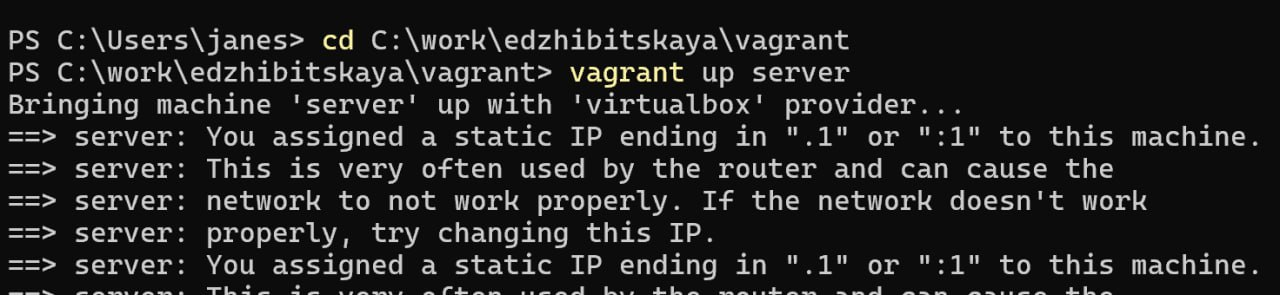
\includegraphics[width=0.7\linewidth,height=\textheight,keepaspectratio]{image/1.jpg}

}

\caption{Запуск ОС}

\end{figure}%

\begin{figure}

{\centering 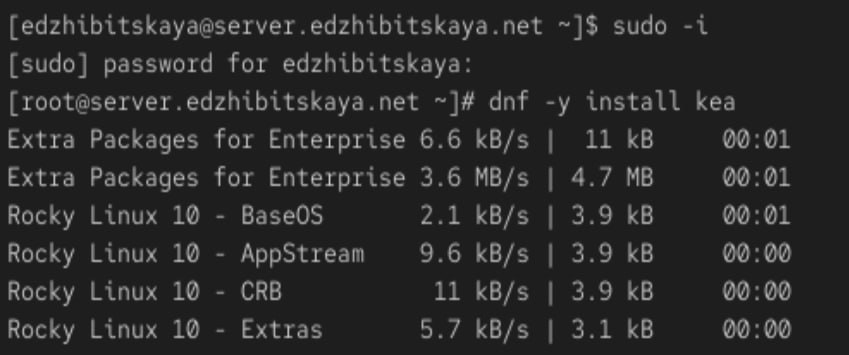
\includegraphics[width=0.7\linewidth,height=\textheight,keepaspectratio]{image/2.jpg}

}

\caption{Установка Kea}

\end{figure}%

На всякий случай сохраняем файл конфигурации(копируем его), открываем на
редактирование и меняем шаблон. Указываем имя, адрес подсети, диапазон
адресов для распределения клиентам, адрес маршрутизатора и
broadcast-адрес. Также настраиваем привязку dhcpd к интерфейсу eth1
(рис. {[}\textbf{fig:003?}{]}, рис. {[}\textbf{fig:004?}{]} и рис.
{[}\textbf{fig:005?}{]}).

\begin{figure}

{\centering 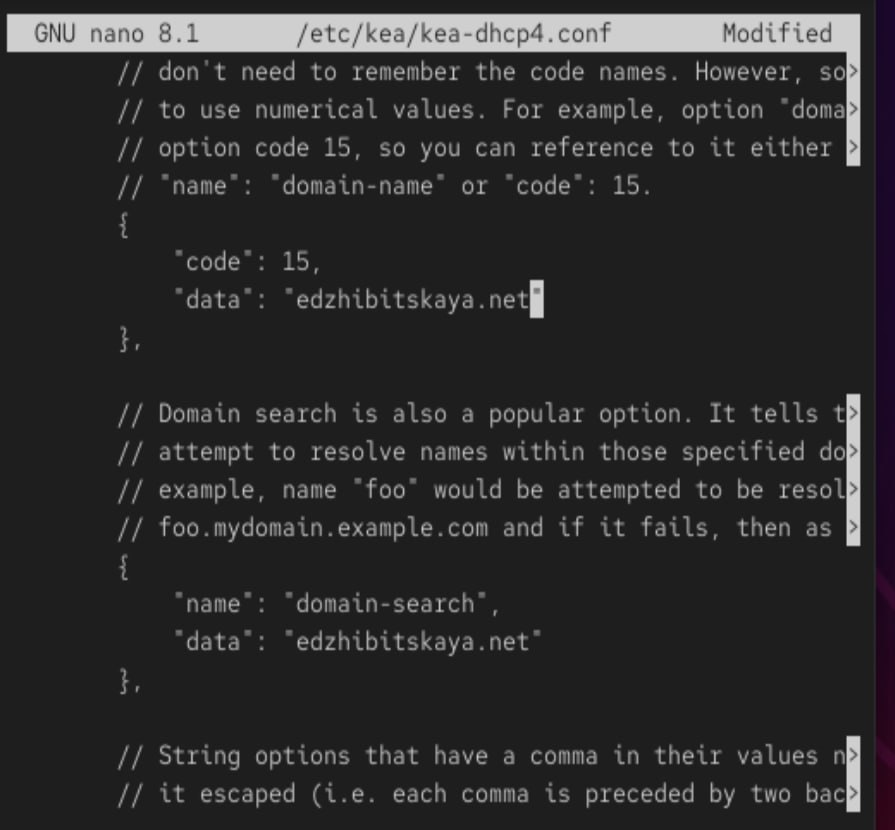
\includegraphics[width=0.7\linewidth,height=\textheight,keepaspectratio]{image/3.jpg}

}

\caption{Настройка файла конфигурации. Domain-name}

\end{figure}%

\begin{figure}

{\centering 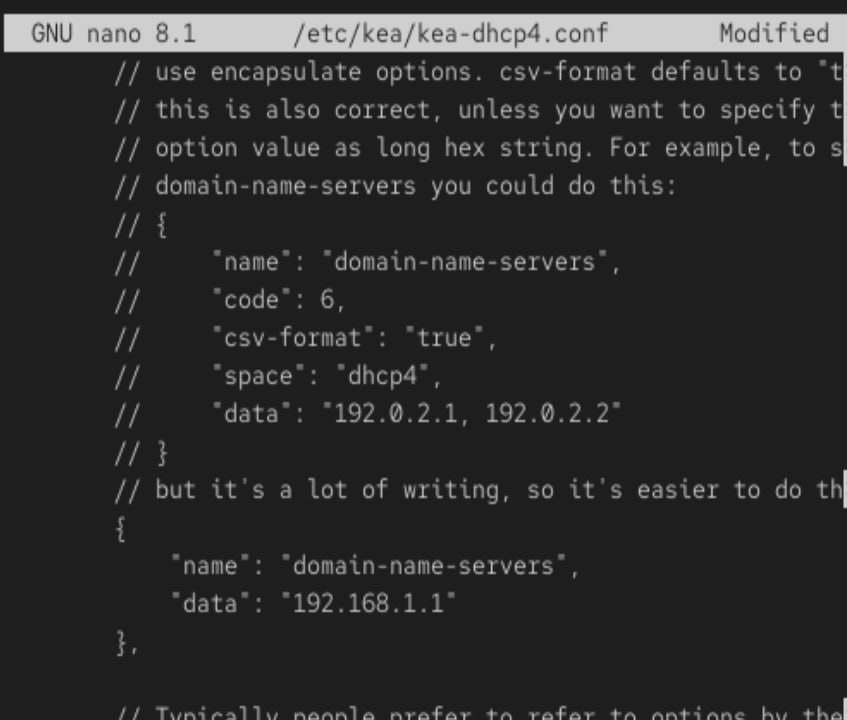
\includegraphics[width=0.7\linewidth,height=\textheight,keepaspectratio]{image/4.jpg}

}

\caption{Domain-name-servers}

\end{figure}%

\begin{figure}

{\centering 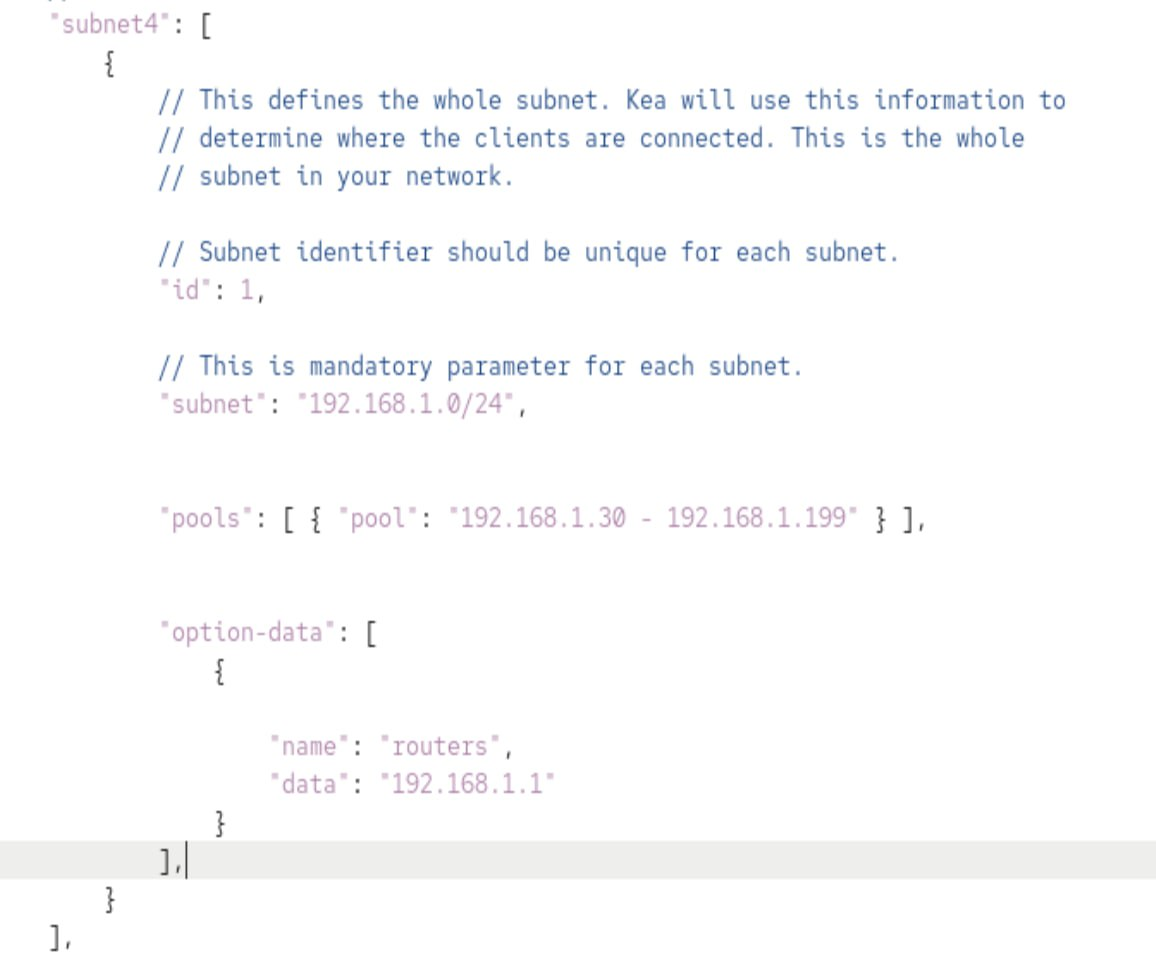
\includegraphics[width=0.7\linewidth,height=\textheight,keepaspectratio]{image/5.jpg}

}

\caption{Subnet4}

\end{figure}%

Проверяем правильность командой ``kea-dhcp4 -t /etc/kea/kea-dhcp4.conf''
и перезапускаем конфигурацию, разрешаем загрузку при запуске (рис.
{[}\textbf{fig:006?}{]}).

\begin{figure}

{\centering 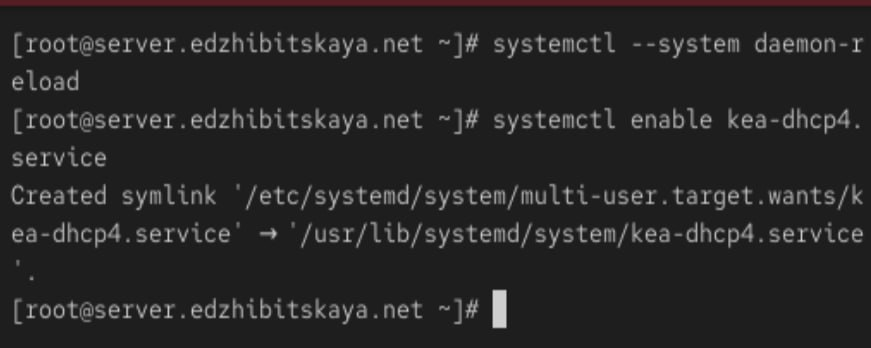
\includegraphics[width=0.7\linewidth,height=\textheight,keepaspectratio]{image/6.jpg}

}

\caption{Перезапуск dhcp}

\end{figure}%

Редактируем файлы прямой DNS-зоны и обратной, добавляем запись для
DHCP-сервер(рис. {[}\textbf{fig:007?}{]} и рис.
{[}\textbf{fig:008?}{]}).

\begin{figure}

{\centering 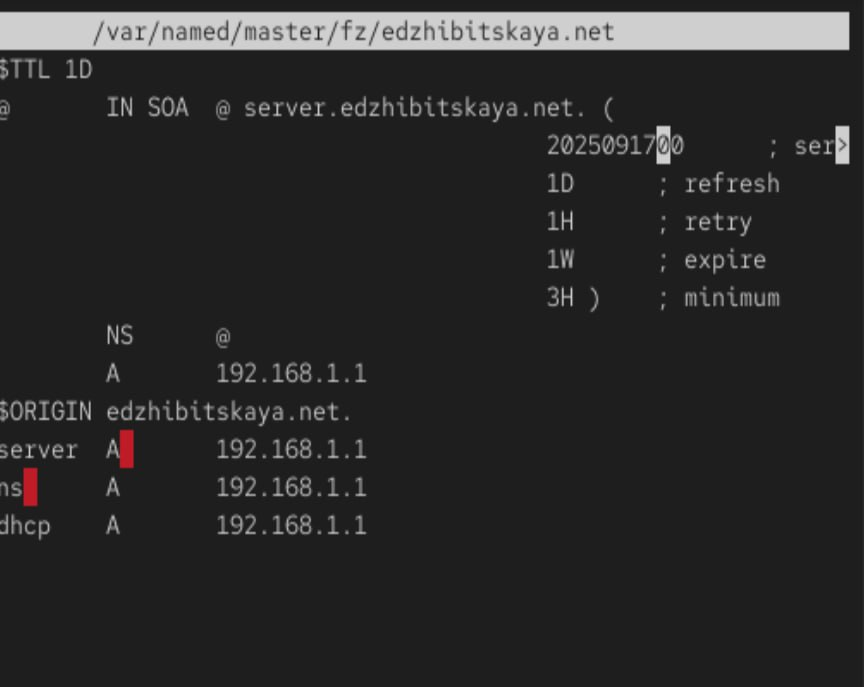
\includegraphics[width=0.7\linewidth,height=\textheight,keepaspectratio]{image/7.jpg}

}

\caption{Файл прямой DNS-зоны}

\end{figure}%

\begin{figure}

{\centering 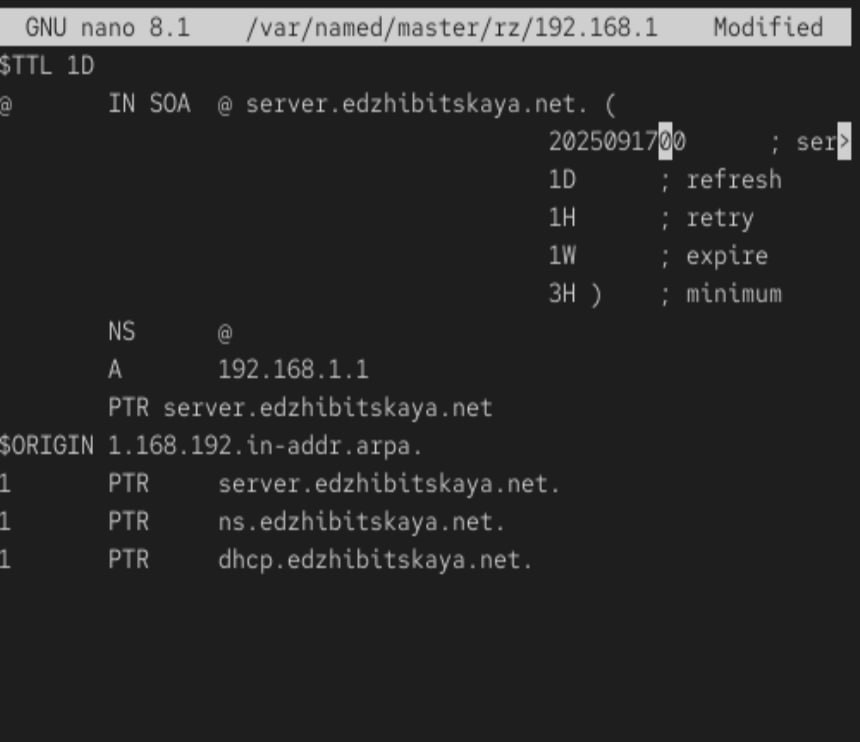
\includegraphics[width=0.7\linewidth,height=\textheight,keepaspectratio]{image/8.jpg}

}

\caption{Файл обратной DNS-зоны}

\end{figure}%

Перезапускаем named, проверяем, что обращение по имени возможно(рис.
{[}\textbf{fig:009?}{]}).

\begin{figure}

{\centering 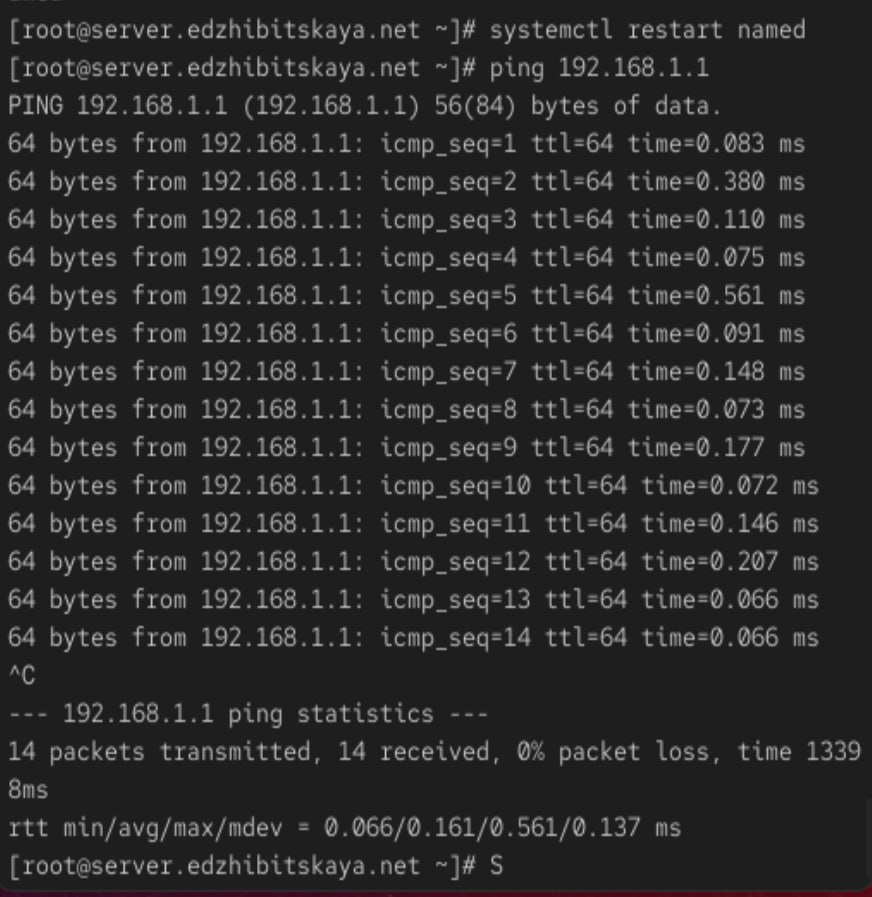
\includegraphics[width=0.7\linewidth,height=\textheight,keepaspectratio]{image/9.jpg}

}

\caption{Обращение к DHCP-серверу по имени}

\end{figure}%

Затем вносим изменения в настройки межсетевого экрана узла server,
разрешив работу с DHCP(рис. {[}\textbf{fig:010?}{]} и рис.
{[}\textbf{fig:011?}{]}) и восстанавливаем контекст безопасности в
SELinux(рис. {[}\textbf{fig:012?}{]})

\begin{figure}

{\centering 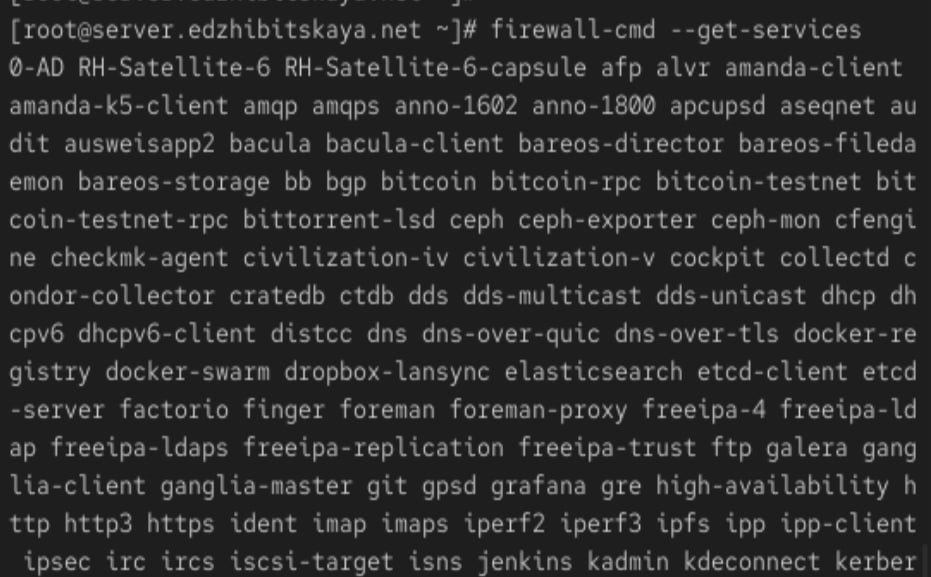
\includegraphics[width=0.7\linewidth,height=\textheight,keepaspectratio]{image/10.jpg}

}

\caption{firewall-cmd --get-services}

\end{figure}%

\begin{figure}

{\centering 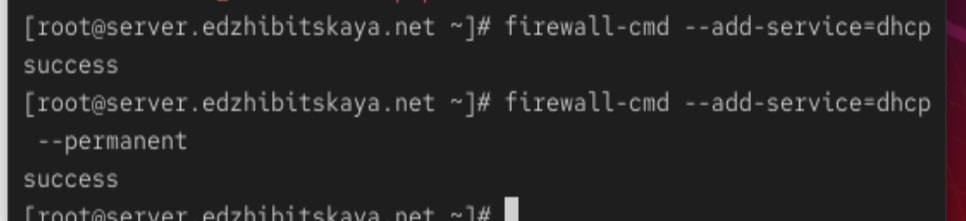
\includegraphics[width=0.7\linewidth,height=\textheight,keepaspectratio]{image/11.jpg}

}

\caption{Добавление dhcp}

\end{figure}%

\begin{figure}

{\centering 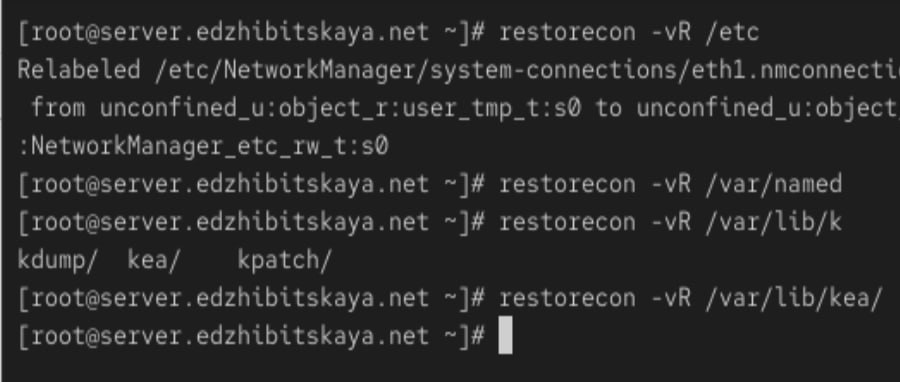
\includegraphics[width=0.7\linewidth,height=\textheight,keepaspectratio]{image/12.jpg}

}

\caption{Восстановление контекста безопасности}

\end{figure}%

Наконец, в еще одном терминале запускаем просмотр лога ошибок, а в
основонм терминале запускаем сам сервис(рис. {[}\textbf{fig:013?}{]}).

\begin{figure}

{\centering 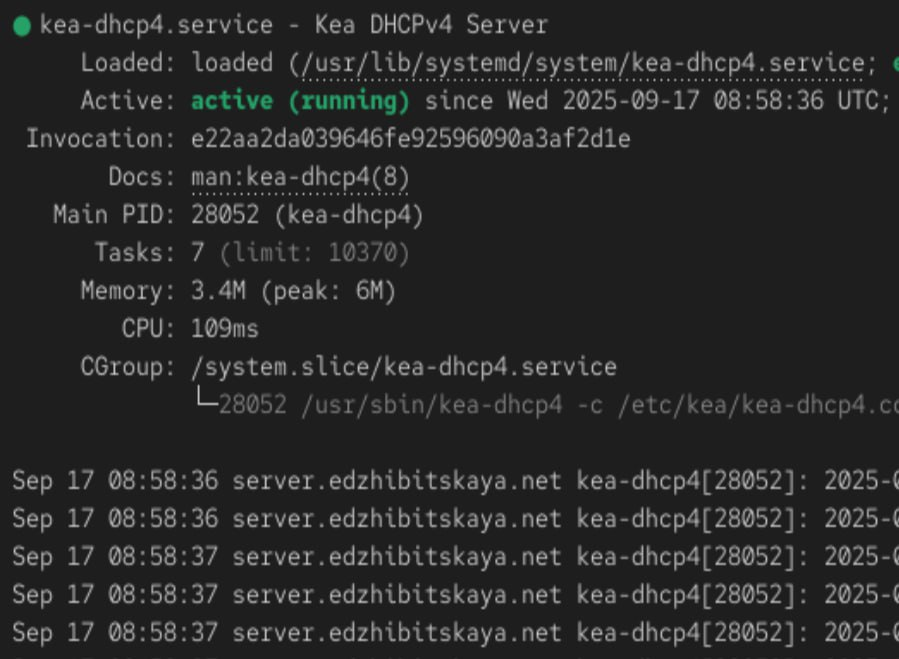
\includegraphics[width=0.7\linewidth,height=\textheight,keepaspectratio]{image/13.jpg}

}

\caption{Запуск dhcp}

\end{figure}%

Переходим к анализу работы сервера.

Перед запуском виртуальной машины client в каталоге с проектом
подкаталоге client создаем файл 01-routing.sh, добавляем скрипт
настройки NetworkManager, чтобы весь трафик client шёл по умолчанию
через eth1(рис. {[}\textbf{fig:014?}{]}). Добавляем соответствущий
скрипт в Vagrantfile(рис. {[}\textbf{fig:015?}{]}).

\begin{figure}

{\centering 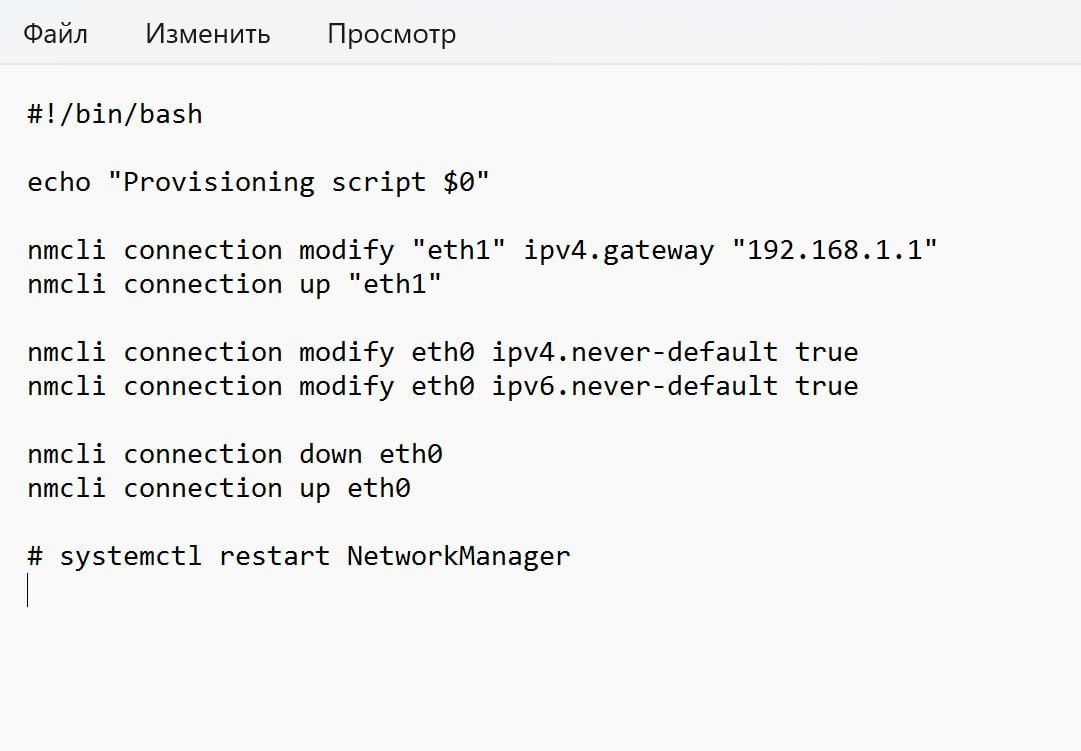
\includegraphics[width=0.7\linewidth,height=\textheight,keepaspectratio]{image/14.jpg}

}

\caption{Файл 01-routing.sh}

\end{figure}%

\begin{figure}

{\centering 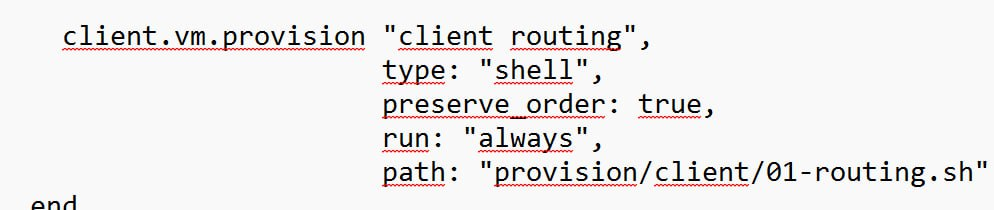
\includegraphics[width=0.7\linewidth,height=\textheight,keepaspectratio]{image/15.jpg}

}

\caption{Vagrantfile}

\end{figure}%

Запускаем машину client с внесенными изменениями(рис.
{[}\textbf{fig:016?}{]}). На машине server на терминале с мониторингом
можно увидеть записи о подключении к виртуальной внутренней сети узла
client и выдачи ему IP-адреса из соответствующего диапазона адресов.

\begin{figure}

{\centering 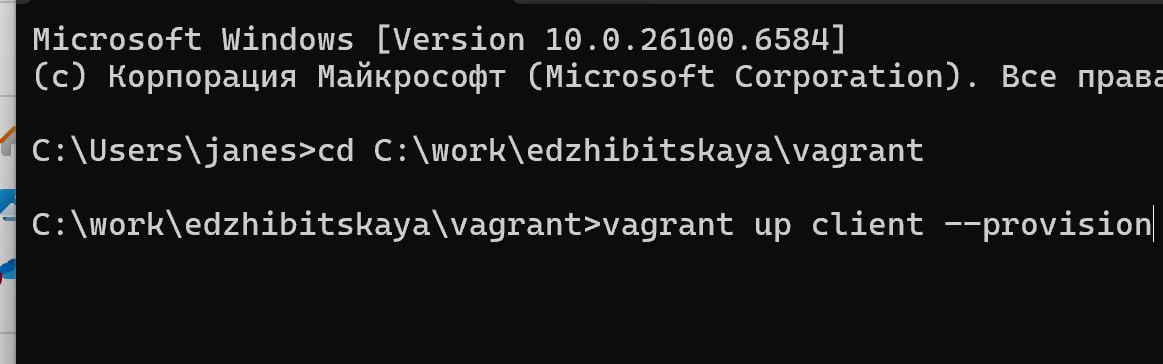
\includegraphics[width=0.7\linewidth,height=\textheight,keepaspectratio]{image/16.jpg}

}

\caption{Запуск client}

\end{figure}%

В терминале запущенной машины смотрим информацию об имеющихся
интерфейсах(рис. {[}\textbf{fig:017?}{]}), а на сервере смотрим список
адресов(рис. {[}\textbf{fig:018?}{]}). Файл хранит информацию о
выделенных DHCP адресах. Записи включают в себя IP-адрес, который был
выделен клиенту, информацию о том кому и на какой срок выдан адрес, дату
начала и окончания, MAC-адрес сетевого интерфейса, который был
использован при получении IP-адреса, идентификатор клиента и имя хоста.

\begin{figure}

{\centering 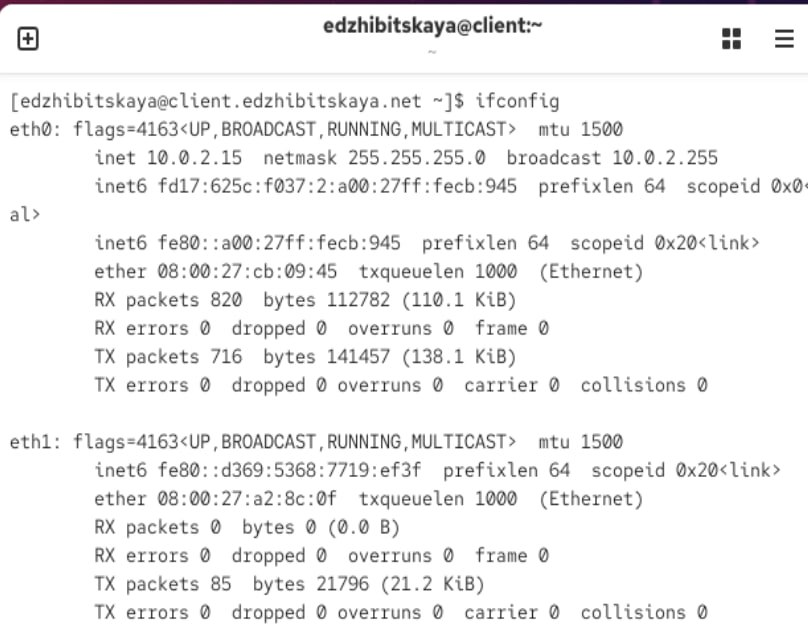
\includegraphics[width=0.7\linewidth,height=\textheight,keepaspectratio]{image/17.jpg}

}

\caption{Интерфейсы}

\end{figure}%

\begin{figure}

{\centering 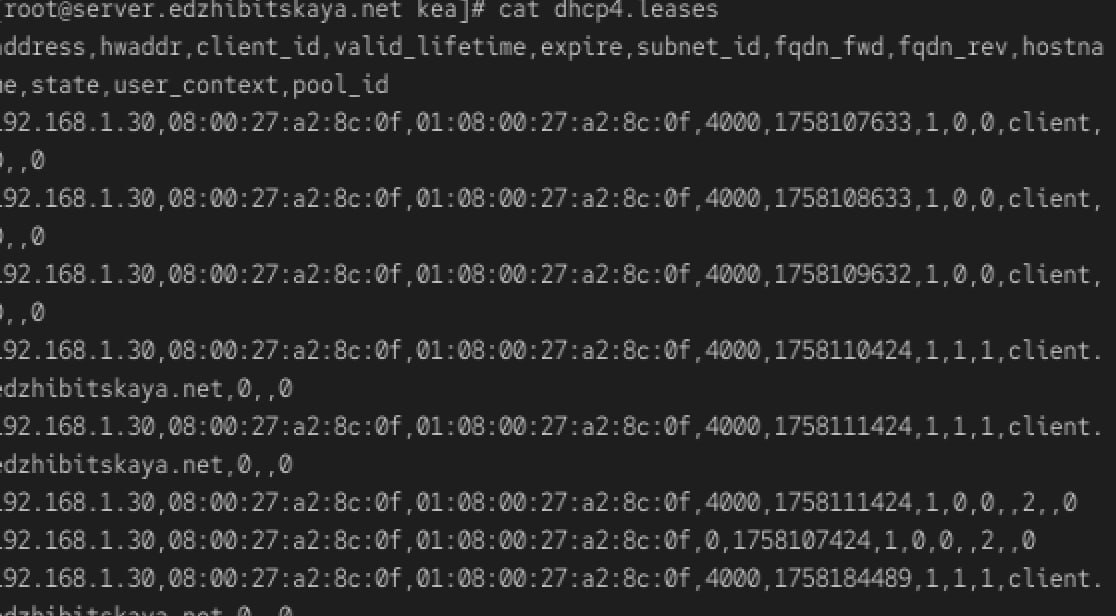
\includegraphics[width=0.7\linewidth,height=\textheight,keepaspectratio]{image/18.jpg}

}

\caption{Выданные адреса}

\end{figure}%

Перейдем к настройке обновления DNS-зоны.

Создаем ключ на сервере с Bind9(рис. {[}\textbf{fig:019?}{]}). Поправим
права доступа и подкючим ключ в файле(рис. {[}\textbf{fig:020?}{]} и
рис. {[}\textbf{fig:021?}{]}).

\begin{figure}

{\centering 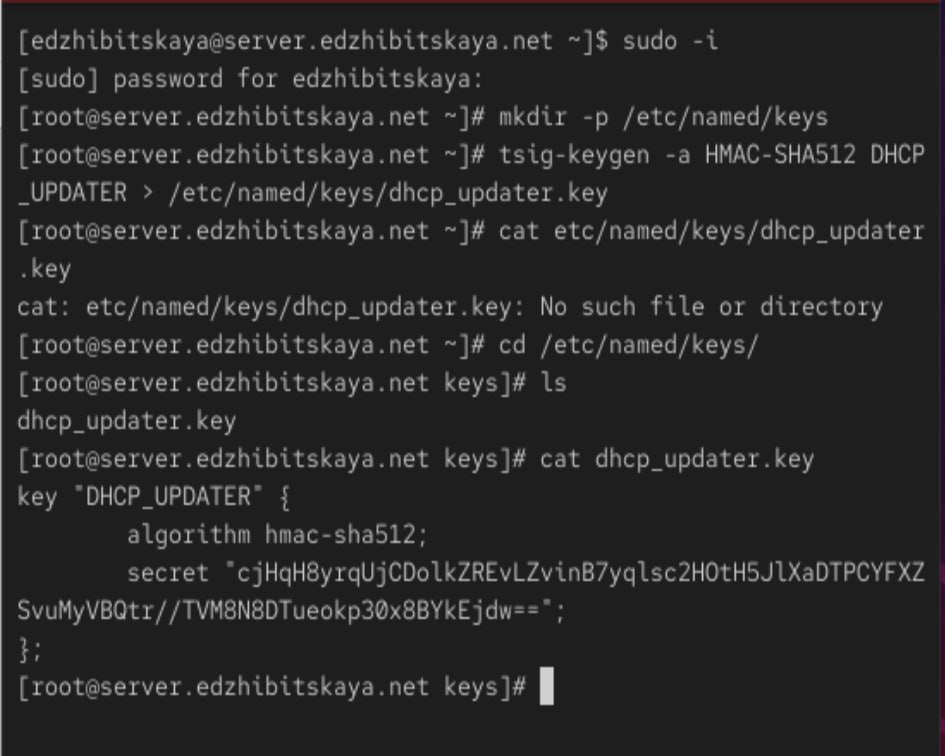
\includegraphics[width=0.7\linewidth,height=\textheight,keepaspectratio]{image/19.jpg}

}

\caption{Создание ключа}

\end{figure}%

\begin{figure}

{\centering 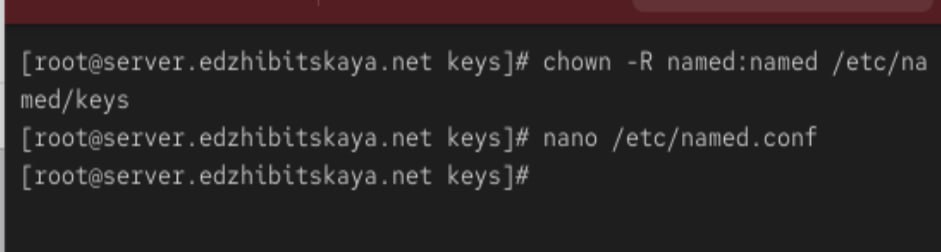
\includegraphics[width=0.7\linewidth,height=\textheight,keepaspectratio]{image/20.jpg}

}

\caption{Права доступа}

\end{figure}%

\begin{figure}

{\centering 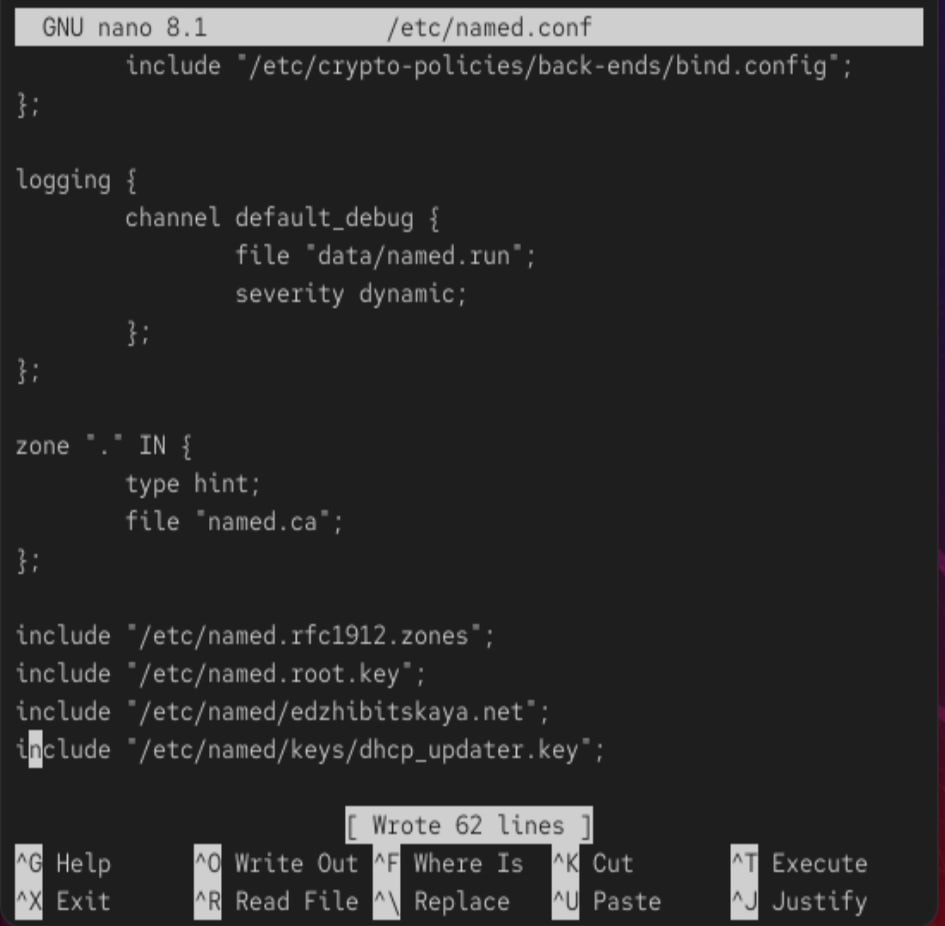
\includegraphics[width=0.7\linewidth,height=\textheight,keepaspectratio]{image/21.jpg}

}

\caption{Подключение в файле}

\end{figure}%

Также разрешим обновление в файле /etc/named/edzhibitskaya.net (рис.
{[}\textbf{fig:022?}{]}).

\begin{figure}

{\centering 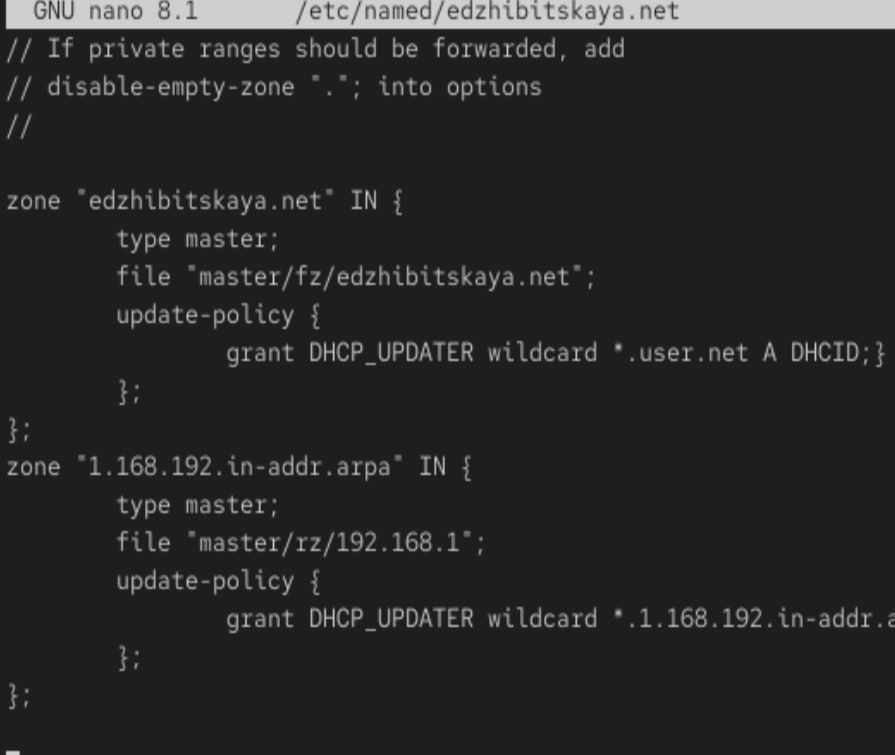
\includegraphics[width=0.7\linewidth,height=\textheight,keepaspectratio]{image/22.jpg}

}

\caption{Разрешение обновления}

\end{figure}%

Проверяем на наличие опечаток, исправялем и перезапускаем named (рис.
{[}\textbf{fig:023?}{]}).

\begin{figure}

{\centering 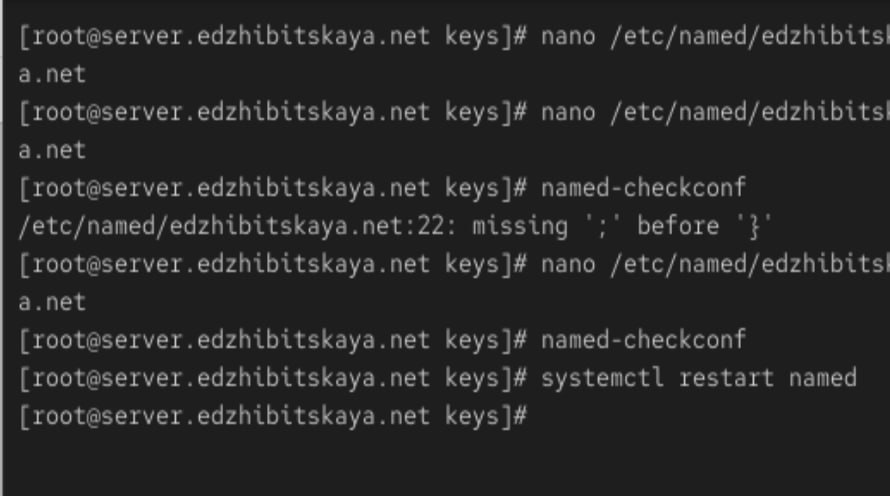
\includegraphics[width=0.7\linewidth,height=\textheight,keepaspectratio]{image/23.jpg}

}

\caption{Перезапуск DNS-сервера}

\end{figure}%

Далее формируем ключ(рис. {[}\textbf{fig:024?}{]}). Меням владельца и
поправляем права доступа.

\begin{figure}

{\centering 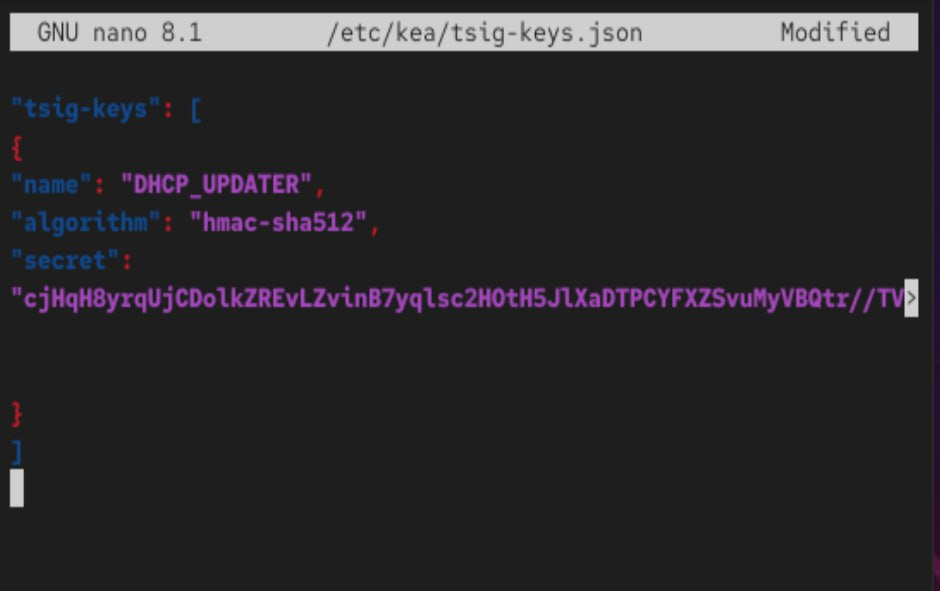
\includegraphics[width=0.7\linewidth,height=\textheight,keepaspectratio]{image/24.jpg}

}

\caption{Формирование ключа}

\end{figure}%

В файле /etc/kea/kea-dhcp-ddns.conf прописываем все настройки(рис.
{[}\textbf{fig:025?}{]}).

\begin{figure}

{\centering 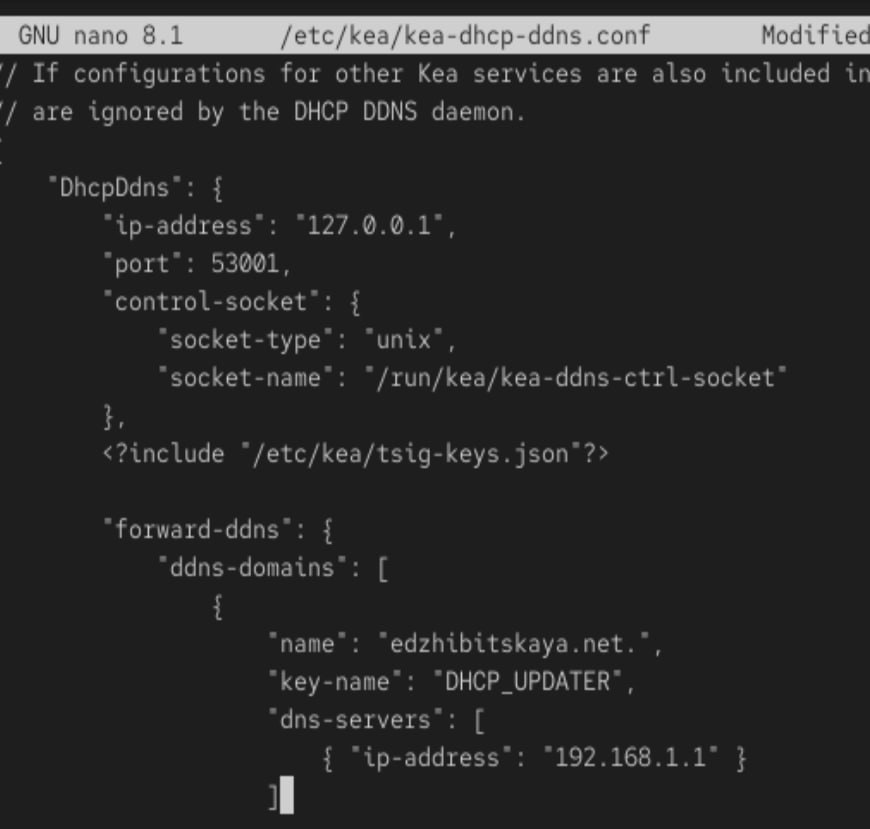
\includegraphics[width=0.7\linewidth,height=\textheight,keepaspectratio]{image/25.jpg}

}

\caption{kea-dhcp-ddns.conf}

\end{figure}%

Проверяем на наличие ошибок, меняем владельца ``chown kea:kea
/etc/kea/kea-dhcp-ddns.conf'' и запускаем службу(рис.
{[}\textbf{fig:026?}{]}).

\begin{figure}

{\centering 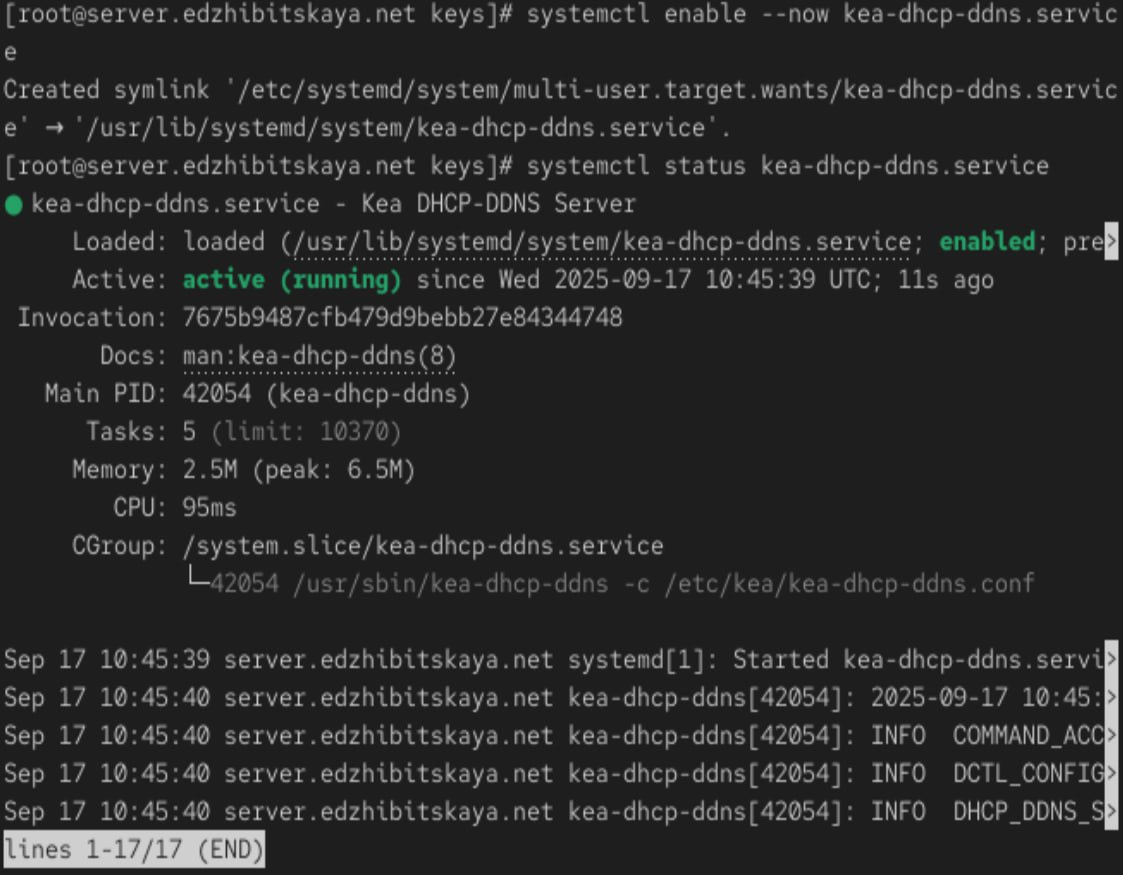
\includegraphics[width=0.7\linewidth,height=\textheight,keepaspectratio]{image/26.jpg}

}

\caption{Запуск dhcp-ddns}

\end{figure}%

Кроме того добавляем изменения в конфигурационный файл
/etc/kea/kea-dhcp4.conf(рис. {[}\textbf{fig:027?}{]}). Проверяем на
наличие ошибок и запускаем сервер(рис. {[}\textbf{fig:028?}{]}).

\begin{figure}

{\centering 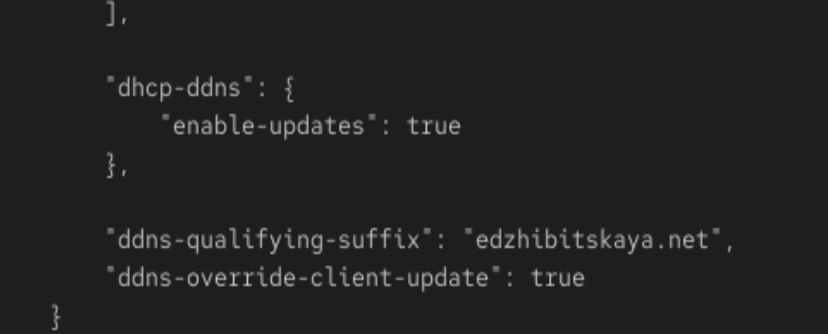
\includegraphics[width=0.7\linewidth,height=\textheight,keepaspectratio]{image/27.jpg}

}

\caption{kea-dhcp4.conf}

\end{figure}%

\begin{figure}

{\centering 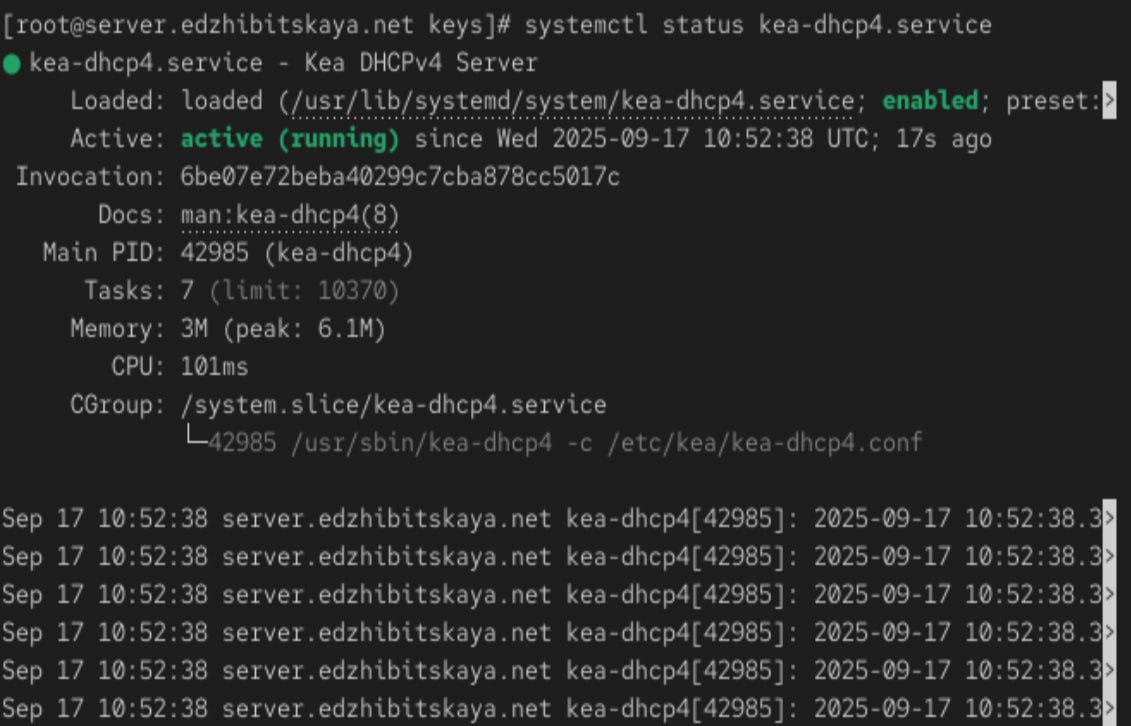
\includegraphics[width=0.7\linewidth,height=\textheight,keepaspectratio]{image/28.jpg}

}

\caption{Запуск dhcp}

\end{figure}%

На машине client переполучаем адрес, в каталоге прямой DNS-зоны
появляется файл edzhibitskaya.net.jnl, в котором автоматически вносятся
изменения записей зоны(рис. {[}\textbf{fig:029?}{]} и рис.
{[}\textbf{fig:030?}{]}).

\begin{figure}

{\centering 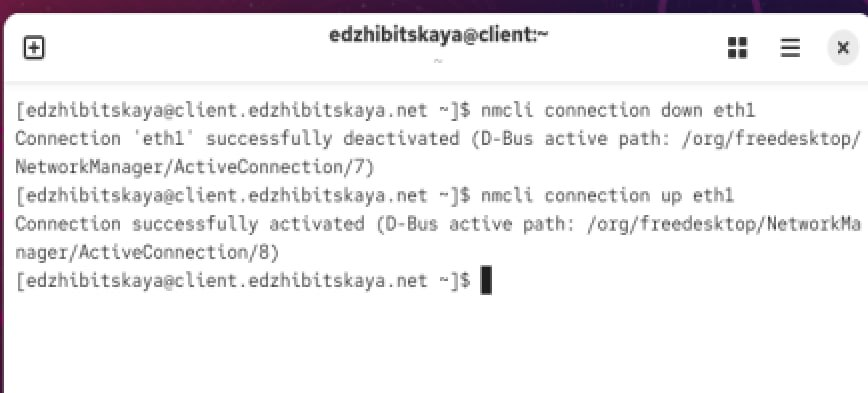
\includegraphics[width=0.7\linewidth,height=\textheight,keepaspectratio]{image/29.jpg}

}

\caption{Переполучение адреса}

\end{figure}%

\begin{figure}

{\centering 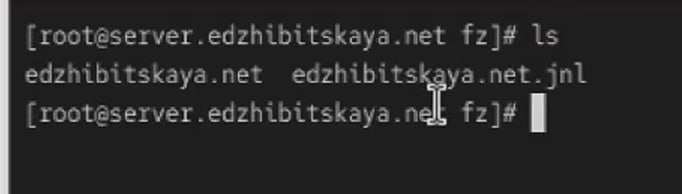
\includegraphics[width=0.7\linewidth,height=\textheight,keepaspectratio]{image/30.jpg}

}

\caption{edzhibitskaya.net.jnl}

\end{figure}%

Анализируем работу DHCP-сервера после настройки обновлений.

На машине client с помощью утилиты dig убедимся в наличии DNS-записи о
клиенте в прямой DNS-зоне( рис. {[}\textbf{fig:031?}{]}).

\begin{figure}

{\centering 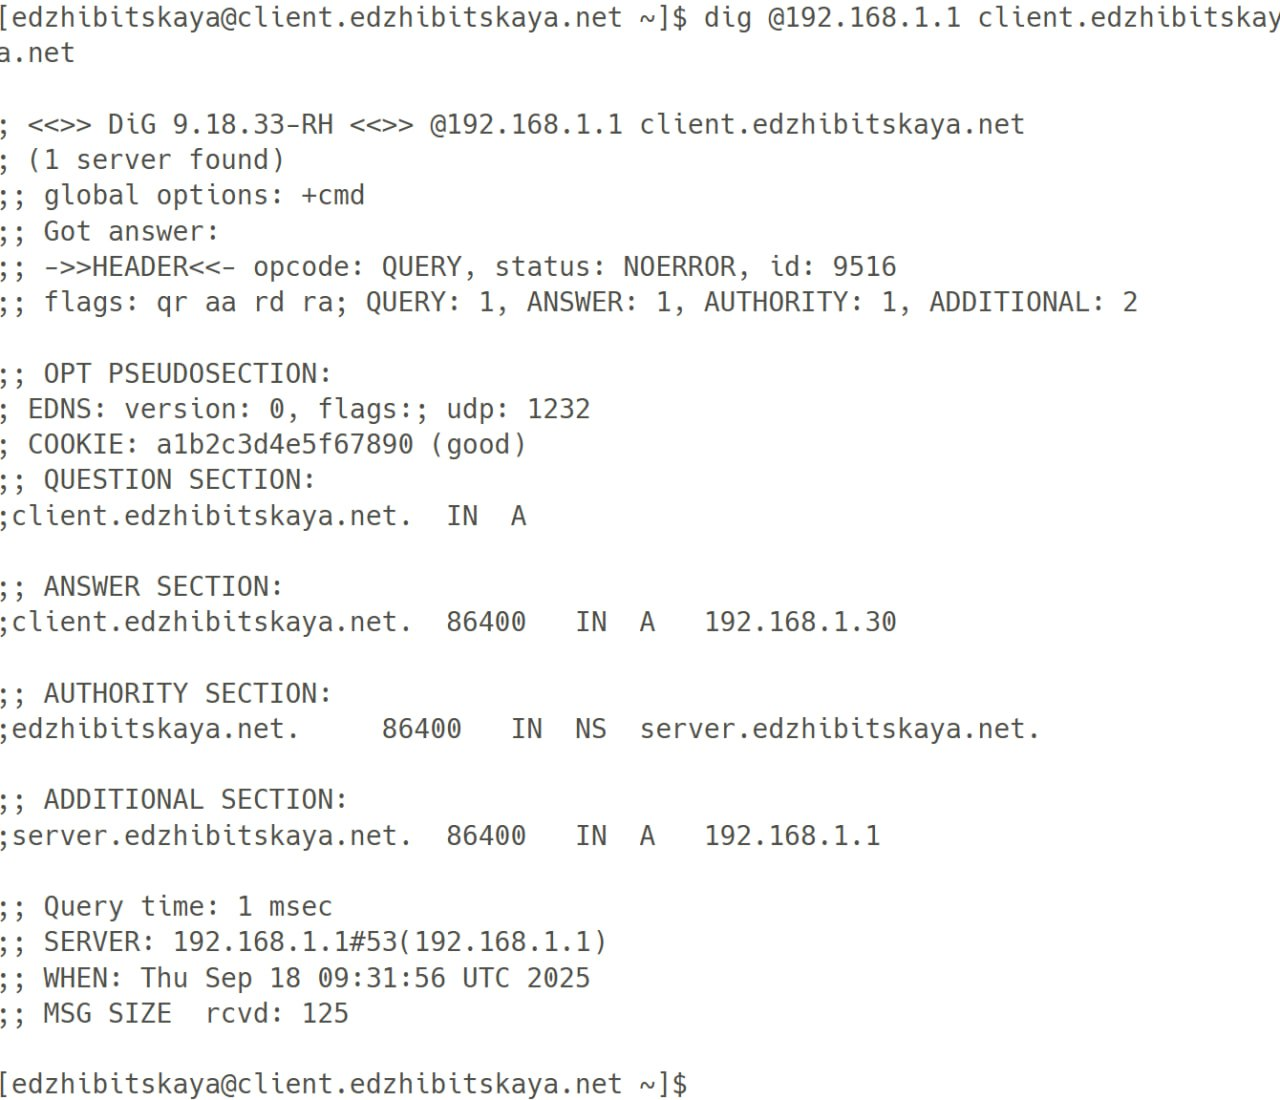
\includegraphics[width=0.7\linewidth,height=\textheight,keepaspectratio]{image/37.jpg}

}

\caption{Запись о клиенте}

\end{figure}%

Наконец внесем изменения в настройки окружения.

На виртуальной машине server в каталог для внесения изменений в
настройки внутреннего окружения /vagrant/provision/server/, создаем
каталог dhcp, в который помещяем соответствующие подкаталоги
конфигурационные файлы DHCP( рис. {[}\textbf{fig:032?}{]}).

\begin{figure}

{\centering 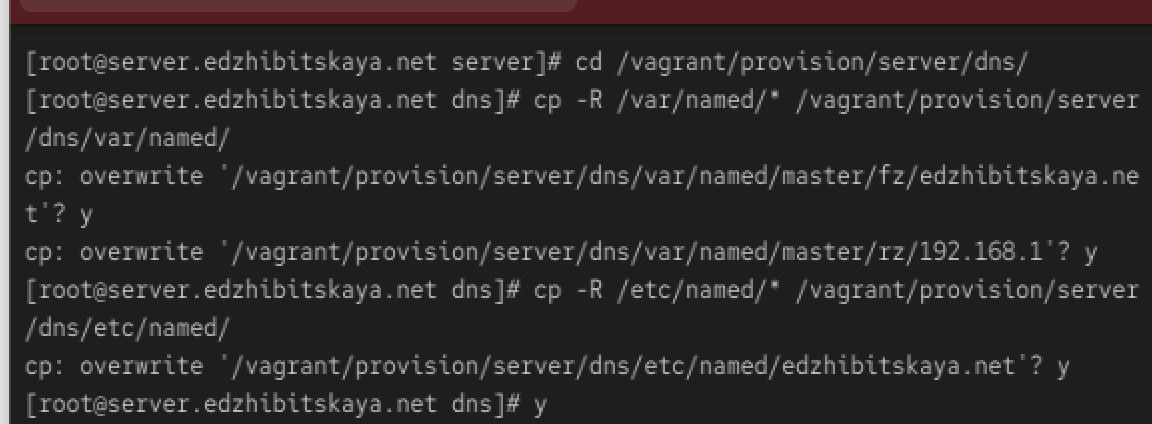
\includegraphics[width=0.7\linewidth,height=\textheight,keepaspectratio]{image/32.jpg}

}

\caption{Каталог DHCP}

\end{figure}%

Затем заменим файл сервера( рис. {[}\textbf{fig:033?}{]}).

\begin{figure}

{\centering 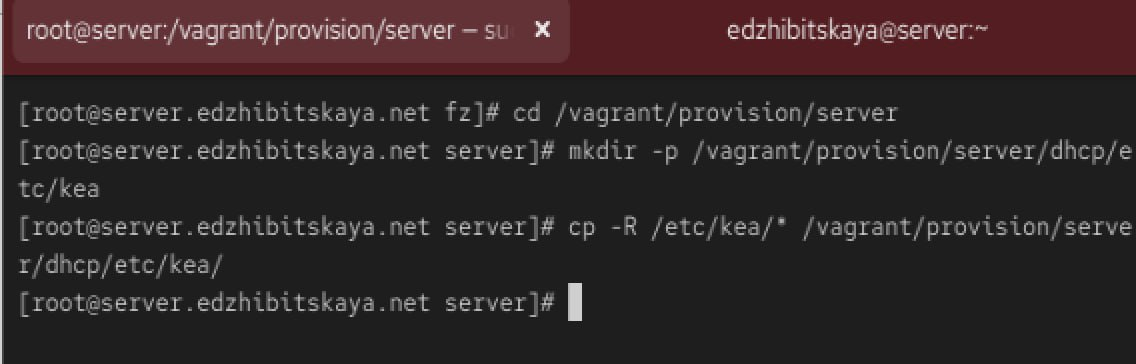
\includegraphics[width=0.7\linewidth,height=\textheight,keepaspectratio]{image/33.jpg}

}

\caption{Замена файлов}

\end{figure}%

Далее создаем файл и добавляем туда скрипт( рис. {[}\textbf{fig:034?}{]}
и рис. {[}\textbf{fig:035?}{]}).

\begin{figure}

{\centering 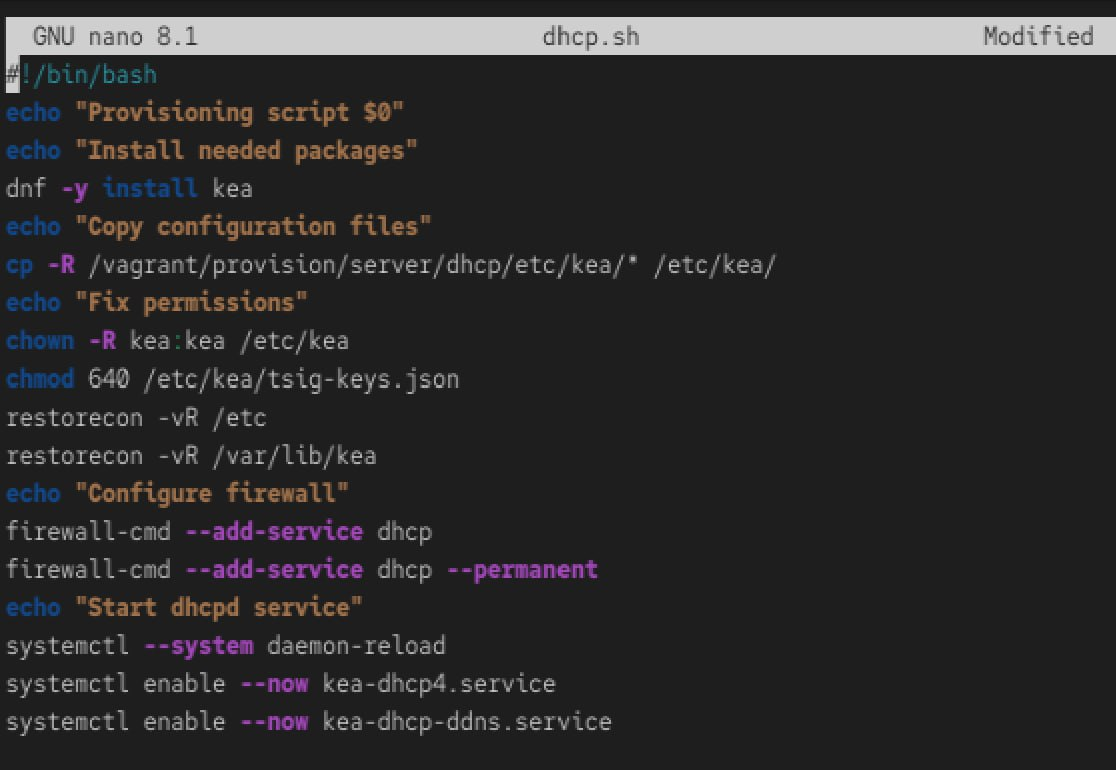
\includegraphics[width=0.7\linewidth,height=\textheight,keepaspectratio]{image/34.jpg}

}

\caption{Создание файла}

\end{figure}%

\begin{figure}

{\centering 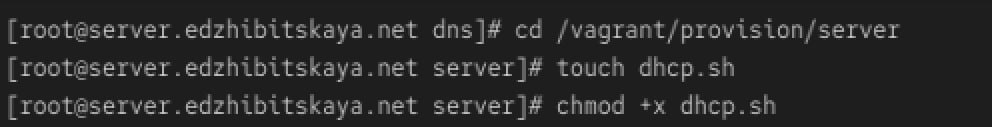
\includegraphics[width=0.7\linewidth,height=\textheight,keepaspectratio]{image/35.jpg}

}

\caption{Файл dhcp.sh}

\end{figure}%

Завершаем работу(рис. {[}\textbf{fig:036?}{]}).

\begin{figure}

{\centering 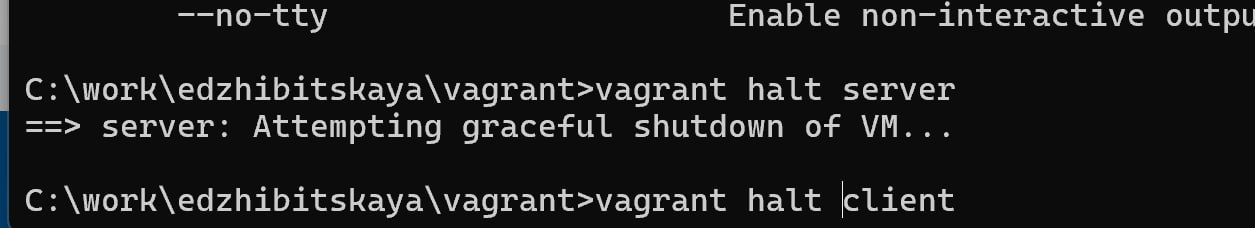
\includegraphics[width=0.7\linewidth,height=\textheight,keepaspectratio]{image/36.jpg}

}

\caption{Выключение}

\end{figure}%

\chapter{Контрольные
вопросы}\label{ux43aux43eux43dux442ux440ux43eux43bux44cux43dux44bux435-ux432ux43eux43fux440ux43eux441ux44b}

\begin{itemize}
\tightlist
\item
  В каких файлах хранятся настройки сетевых подключений?
\end{itemize}

/etc/NetworkManager/system-connections/ (управляется через
NetworkManager)

\begin{itemize}
\tightlist
\item
  За что отвечает протокол DHCP?
\end{itemize}

DHCP (Dynamic Host Configuration Protocol) отвечает за автоматическую
выдачу клиентам сетевых настроек: IP-адреса, маски подсети, шлюза по
умолчанию и адресов DNS-серверов.

\begin{itemize}
\tightlist
\item
  Поясните принцип работы протокола DHCP. Какими сообщениями
  обмениваются клиент и сервер, используя протокол DHCP?
\end{itemize}

Он выделяет каждому компьютеру произвольный свободный IP-адрес из
определённого администратором диапазона

\begin{itemize}
\tightlist
\item
  В каких файлах обычно находятся настройки DHCP-сервера? За что
  отвечает каждый из файлов?
\end{itemize}

/etc/dhcp/dhcpd.conf- содержит все настройки --- объявление подсетей,
пулы адресов, шлюзы, DNS-серверы, время аренды и т.д.

/var/lib/dhcp/dhcpd.leases - автоматически ведется демоном dhcpd, хранит
историю выданных адресов, кому и на какой срок.

\begin{itemize}
\tightlist
\item
  Что такое DDNS? Для чего применяется DDNS?
\end{itemize}

Это технология, позволяющая автоматически обновлять записи на
DNS-сервере в реальном времени

\begin{itemize}
\tightlist
\item
  Какую информацию можно получить, используя утилиту ifconfig? Приведите
  примеры с использованием различных опций.
\end{itemize}

Показывает конфигурацию сетевых интерфейсов (IP-адрес, маску,
MAC-адрес), статистику по приему/передаче данных (RX/TX).

ifconfig -- показать все активные интерфейсы.

ifconfig eth0 -- показать информацию только для интерфейса eth0.

ifconfig eth0 up -- включить (up) интерфейс eth0.

\begin{itemize}
\tightlist
\item
  Какую информацию можно получить, используя утилиту ping?
\end{itemize}

Проверяет доступность узла в сети и качество соединения (время отклика,
потерю пакетов).

\chapter{Выводы}\label{ux432ux44bux432ux43eux434ux44b}

В ходе работы были изучены принципы работы DHCP и приобретены навыки по
установке и конфигурированию DHCP-сервера.

\chapter*{Список
литературы}\label{ux441ux43fux438ux441ux43eux43a-ux43bux438ux442ux435ux440ux430ux442ux443ux440ux44b}
\addcontentsline{toc}{chapter}{Список литературы}

{[}ТУИС{]}
(https://esystem.rudn.ru/pluginfile.php/2854738/mod\_resource/content/8/003-dhcp.pdf)


\printbibliography



\end{document}
